\documentclass{beamer}
\usetheme{default}
\usepackage{centernot}

\newcommand{\op}{\diamond}


\title{Magma equations}

\author{Matthew Bolan, Jose Brox, Mario Carneiro, Martin Dvo\v{r}\'ak, Andr\'es Goens, Harald Husum, Zoltan Kocsis, Alex Meiburg, Pietro Monticone, David Renshaw, Cody Roux, J\'er\'emy~Scanvic, Shreyas Srinivas, Anand Rao Tadipatri, Terence Tao, Vlad Tsyrklevich, Daniel Weber, Fan Zheng,\\et al.}

\date{2025-01-28}


\begin{document}

\begin{frame}[plain]
\maketitle
\end{frame}


\begin{frame}{Mathoverflow question}
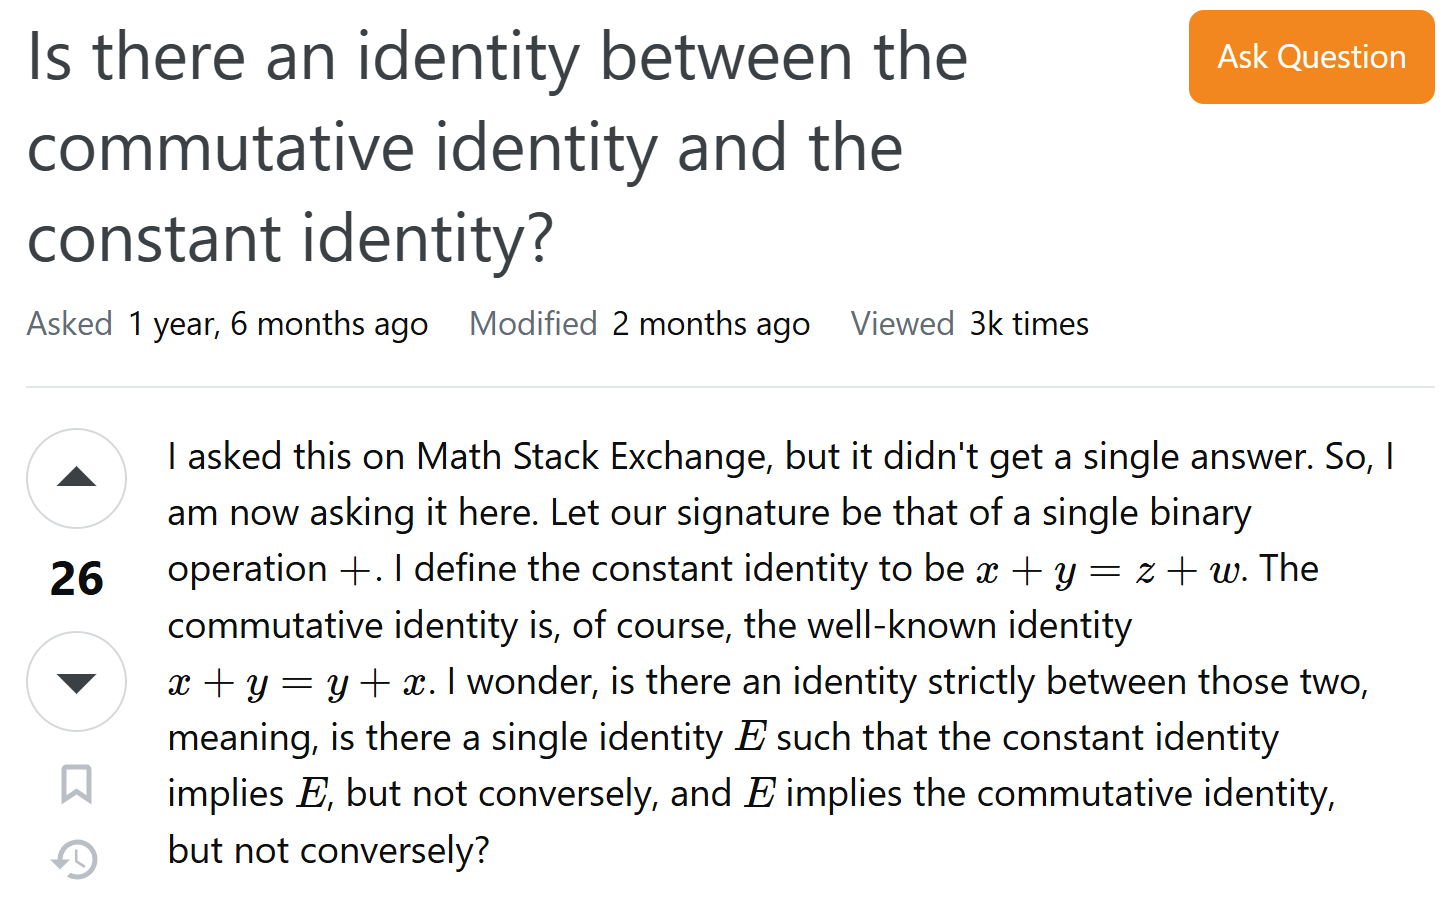
\includegraphics[width=\textwidth]{mathoverflow}
\end{frame}


\begin{frame}{Mathoverflow answer --- before the project started}
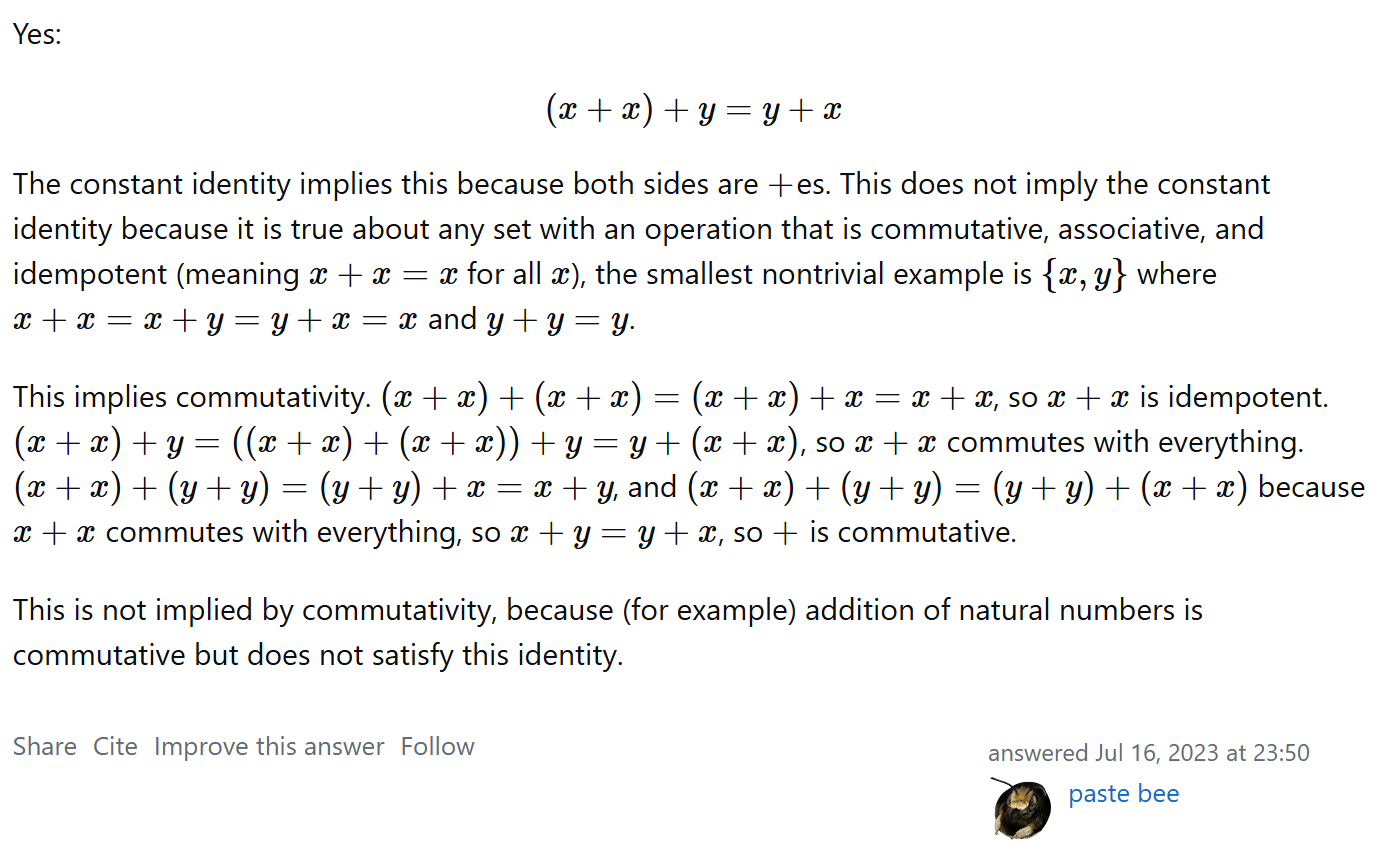
\includegraphics[width=\textwidth]{mathoverflow_bee}
\end{frame}


\begin{frame}{Mathoverflow answer --- after the project started}
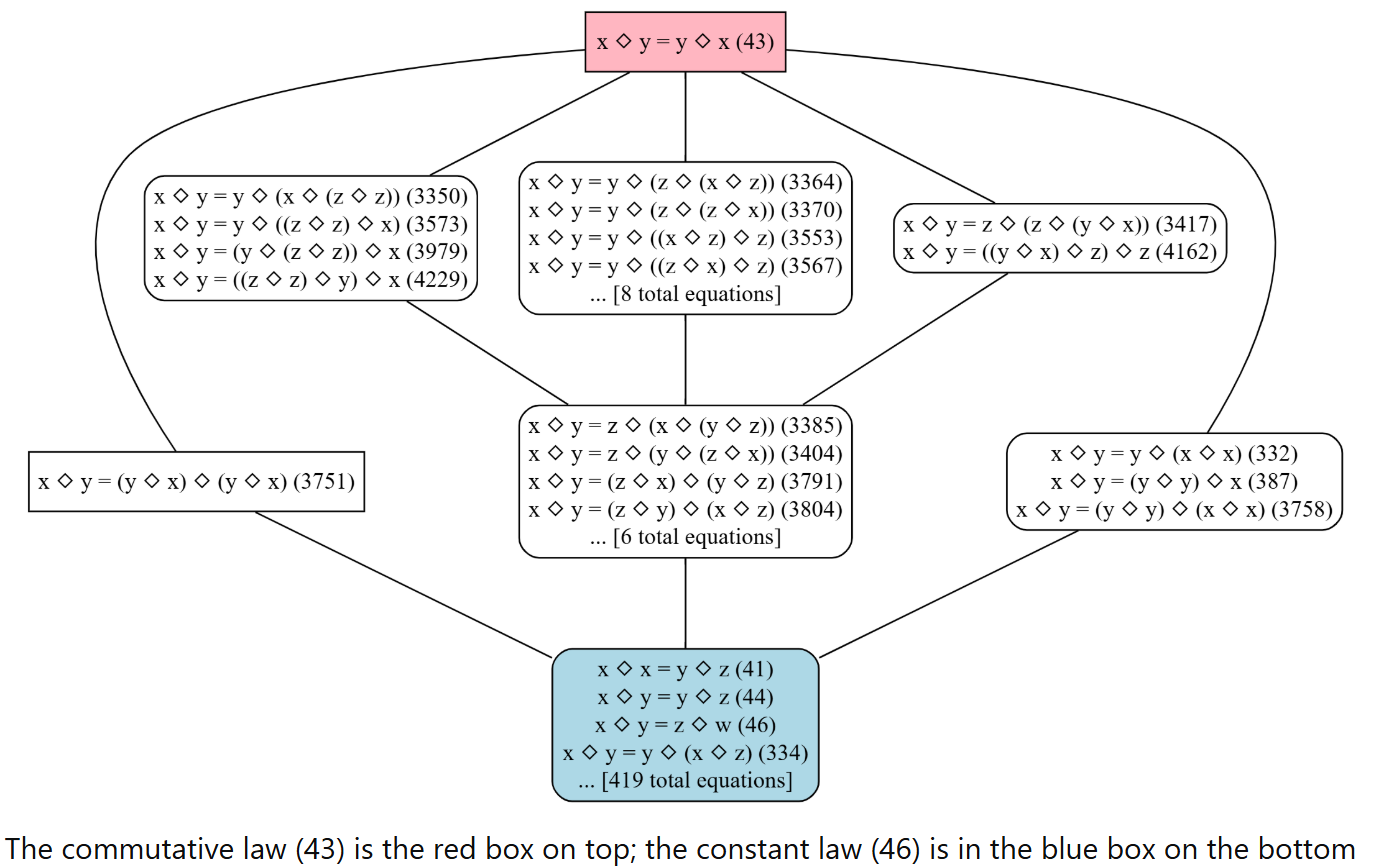
\includegraphics[width=\textwidth]{mathoverflow_tao}
\end{frame}


\begin{frame}{Announcement}
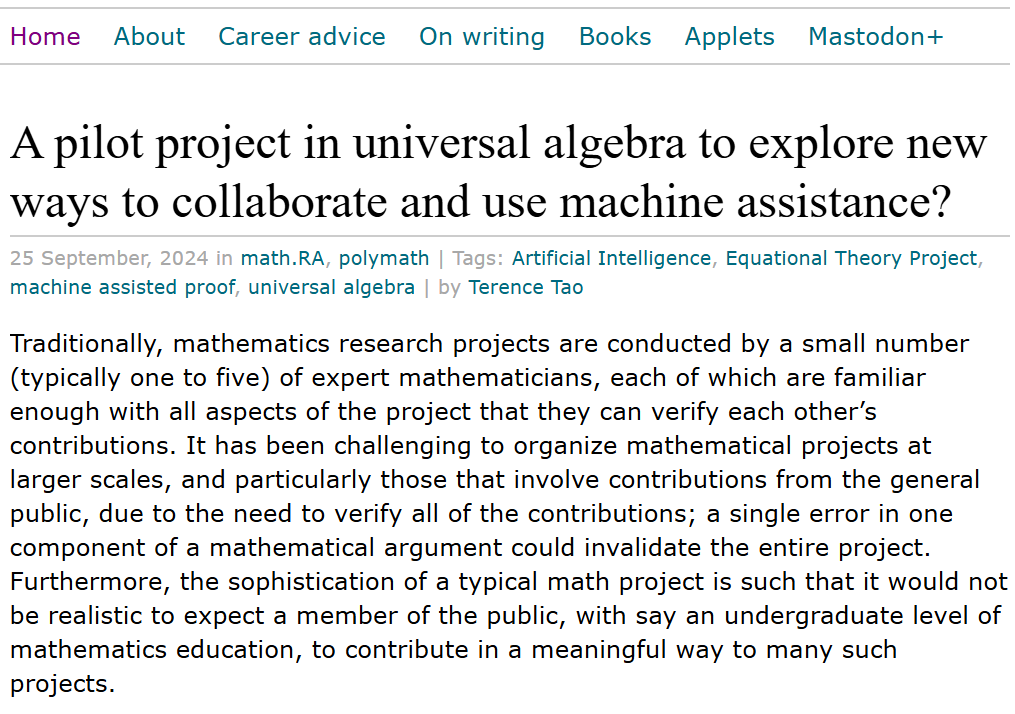
\includegraphics[width=\textwidth]{initial_announcement}
\end{frame}


\begin{frame}{Announcement}
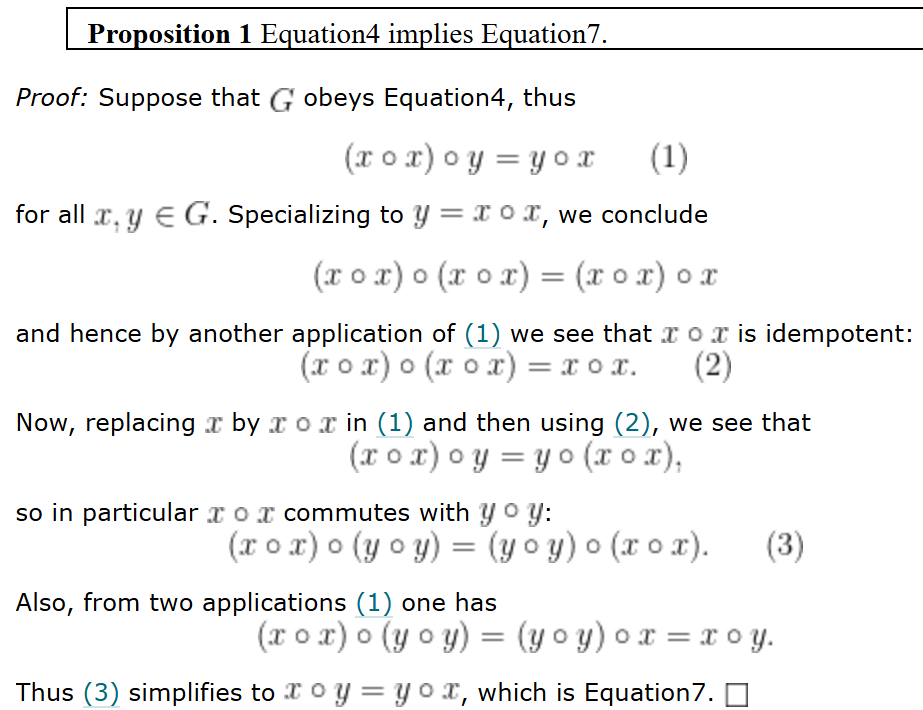
\includegraphics[width=\textwidth]{initial_implication}
\end{frame}


\begin{frame}{Announcement}
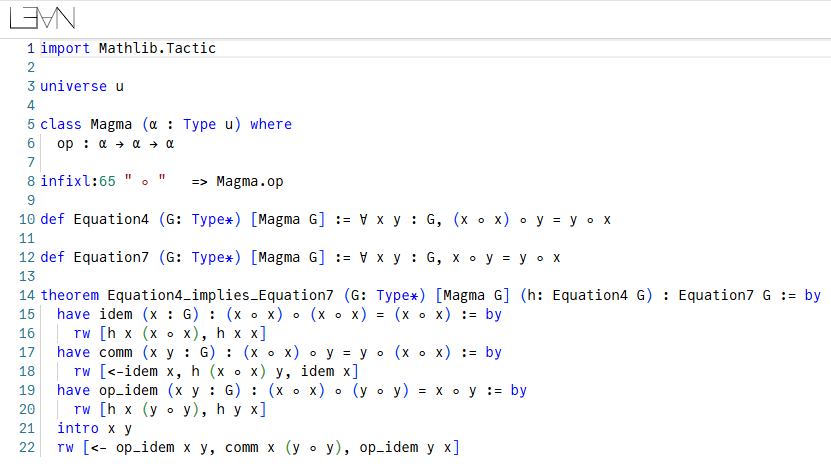
\includegraphics[width=\textwidth]{initial_lean}
\end{frame}


\begin{frame}{Easy implication}
Prove that
$$ \forall x, \forall y,\quad x = x \op y $$
implies
$$ \forall x, \forall y, \forall z, \forall w,\quad x \op y = (x \op z)  \op (w \op y) $$
.

\pause
Solution:
$$ x \op y = x = x \op z = (x \op z) \op (w \op y) $$
\end{frame}


\begin{frame}{Easy counterexample}
Show that
$$ todo $$
does not imply
$$ todo $$
.

\pause
Solution:
$$ todo $$
\end{frame}


\begin{frame}{Why equations?}

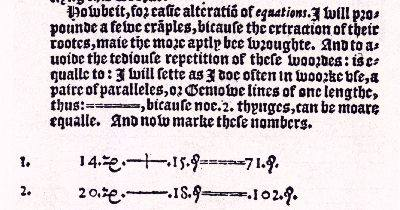
\includegraphics[width=\textwidth]{eq_sign.png}
``I will sette as I doe often in woorke use, a paire of paralleles, or twin lines of one lengthe, thus: =, bicause noe 2 thynges can be moare equalle.''

Robert Recorde's mathematical book The Whetstone of Witte (1557)

\end{frame}


\begin{frame}{Why magmas?}
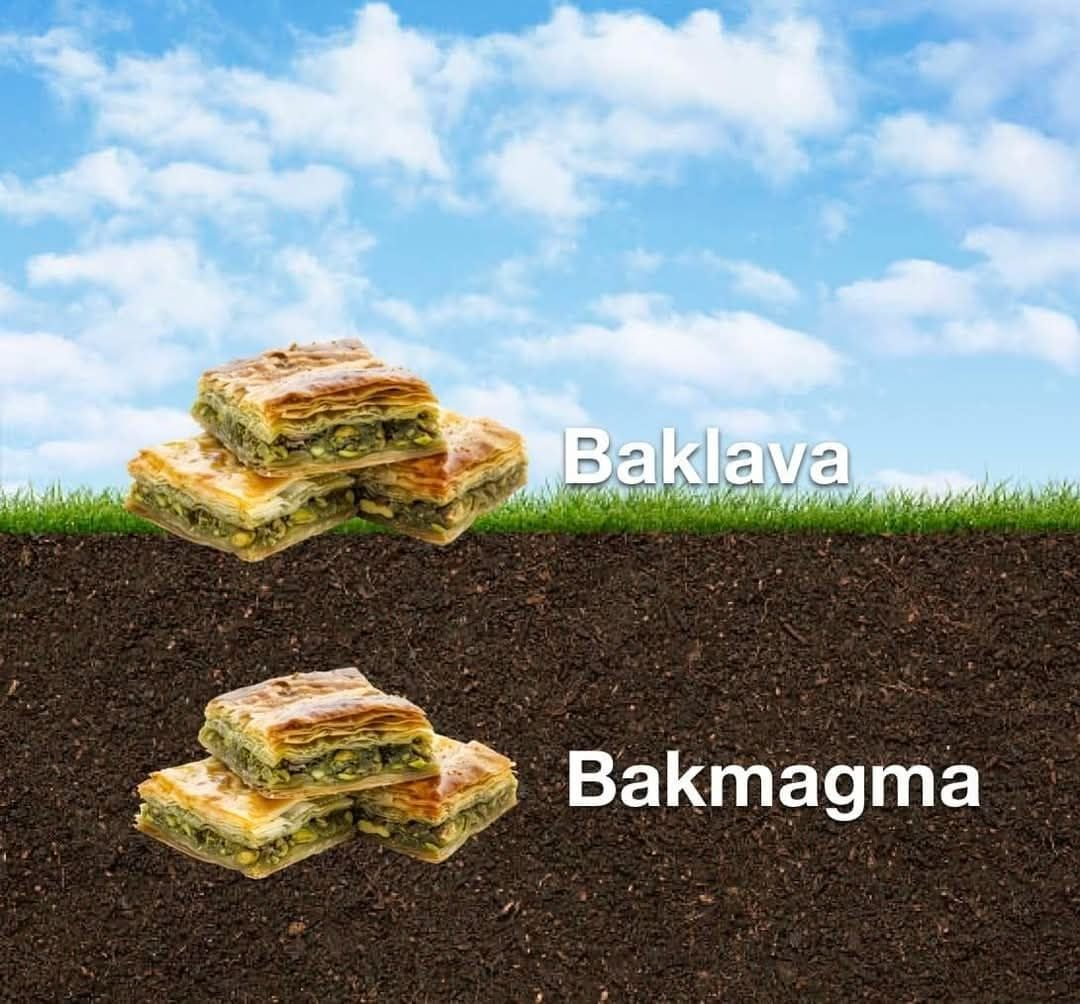
\includegraphics[width=0.8\textwidth]{baklava}
\end{frame}


\begin{frame}{Scope of the project}

Order-0 equations:\vspace*{-1mm}
\[ x = x \tag{E1} \]
\[ x = y \tag{E2} \]
Order-1 equations e.g.:\vspace*{-1mm}
\[ x = y \op z \tag{E7} \]
Order-2 equations e.g.:\vspace*{-3mm}
\[ x \op y = y \op x \tag{E43} \]
Order-3 equations e.g.:\vspace*{-2mm}
\[ x = (y \op x) \op (x \op z) \tag{E168} \]
Order-4 equations e.g.:\vspace*{-2mm}
\[ (x \op y) \op z = (u \op v) \op w \tag{E4694} \]

\end{frame}


\begin{frame}{Lean and manual vs automated contributions}
\end{frame}


\begin{frame}{Implication graph completion}
\begin{itemize}
	\item If $P \implies Q$ and $Q \implies R$, then $P \implies R$.
	\item If $P \implies Q$ and $P \centernot\implies R$, then $Q \centernot\implies R$.
	\item If $Q \implies R$ and $P \centernot\implies R$, then $P \centernot\implies Q$.
\end{itemize}
\end{frame}


\begin{frame}{Constructivism?}

\includegraphics[width=0.6\textwidth]{intuitionists}
\end{frame}


\begin{frame}{Dashboard}
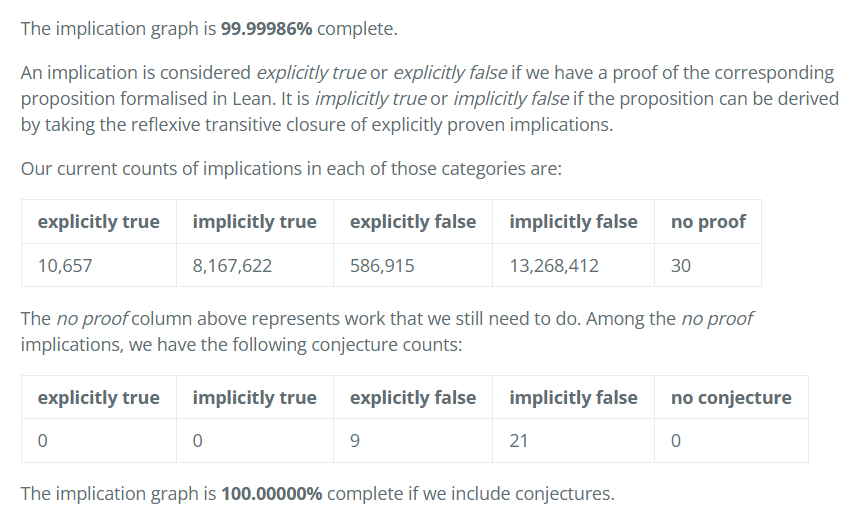
\includegraphics[width=\textwidth]{dashboard}
\end{frame}


\begin{frame}{Equation explorer}
\end{frame}


\begin{frame}{Difficult implication}

Prove that
$$ \forall x, \forall y,\forall z,\quad x = y \op ((x \op x) \op (z \op z)) $$
implies
$$ \forall x_1, \forall y_1,\quad x_1 = y_1 $$
.

\pause
Solution (found by egg):\smallskip

let $x_2 := x_1 \op x_1$

let $x_4 := x_2 \op x_2$

let $x_8 := x_4 \op x_4$

let $y_2 := y_1 \op y_1$

let $y_4 := y_2 \op y_2$

let $y_8 := y_4 \op y_4$

\end{frame}


\begin{frame}{Difficult implication}

\texttt{ass :   }
$ \forall x, \forall y,\forall z,\quad x = y \op ((x \op x) \op (z \op z)) $
\bigskip

Solution (found by egg):\vspace*{-1mm}
$$
\begin{aligned}
	x_1 & = y_1 \op x_4                 && \qquad \qquad \texttt{ass }x_1\ y_1\ x_1 \\
	& = y_1 \op (y_1 \op (x_8 \op x_8)) && \qquad \qquad \texttt{ass }x_4\ y_1\ x_4 \\
	& = y_1 \op (y_1 \op (x_1 \op x_1)) && \qquad \qquad \texttt{ass }x_1\ x_4\ x_1 \\
	& = y_1 \op (y_8 \op (x_1 \op x_1)) && \qquad \qquad \texttt{ass }y_1\ y_4\ y_1 \\
	& = y_4                             && \qquad \qquad \texttt{ass }y_4\ y_1\ x_1 \\
	& = y_1 \op (y_8 \op (y_1 \op y_1)) && \qquad \qquad \texttt{ass }y_4\ y_1\ y_1 \\
	& = y_1 \op (y_1 \op (y_1 \op y_1)) && \qquad \qquad \texttt{ass }y_1\ y_4\ y_1 \\
	& = y_1 \op (y_1 \op (y_8 \op y_8)) && \qquad \qquad \texttt{ass }y_1\ y_4\ y_1 \\
	& = y_1 \op y_4                     && \qquad \qquad \texttt{ass }y_4\ y_1\ y_4 \\
	& = y_1                             && \qquad \qquad \texttt{ass }y_1\ y_1\ y_1
\end{aligned}
$$

\end{frame}


\begin{frame}{Metatheorems}
\end{frame}


\begin{frame}{Counterexample constructions}

\begin{itemize}
	\item Finite magmas
	\item Linear models
	\item Translation-invariant models
	\item Twisting semigroups
	\item Greedy constructions
	\item Ad-hoc modifications
	\item Combinations of the above
\end{itemize}

\end{frame}


\begin{frame}{Greedy constructions}{Preliminaries}

We want to build a magma operation $\op \colon M \times M \to M$ that obeys one equation $E$ but not another $E'$.

We one can first consider \emph{partial magma operations} $\op \colon \Omega \to M$ defined on some  $\Omega \subseteq M \times M$.

We say that a partial operation $\op' \colon \Omega' \to M$ \emph{extends} $\op \colon \Omega \to M$ iff:\!
\begin{itemize}
	\item $\Omega \subseteq \Omega'$
	\item $(x, y) \in \Omega \implies x \op y = x \op' y$
\end{itemize}

Given a sequence $\op_n \colon \Omega_n \to M$ of partial operations, each of which is an extension of the previous, we can define the \emph{direct limit} $\op_\infty \colon \bigcup_n \Omega_n \to M$ to be the partial operation defined by $x \op_\infty y := x \op_n y$ whenever $(x,y) \in \Omega_n$.

\end{frame}


\begin{frame}{Greedy constructions}{Abstract greedy algorithm}
	
Let $E$ and $E'$ be equations.
Let $\Gamma$ be a first-order theory regarding a partial magma operations $\op \colon \Omega \to M$ on a carrier $M$.
Assume the following:
\begin{itemize}
	\item (Seed) There exists a finitely supported partial magma operation $\op_0 \colon \Omega_0 \to M$ satisfying $\Gamma$ that contradicts $E'$, in the sense that there is some assignment of variables in $E'$ in $M$ such that both sides of $E'$ are defined using $\op_0$ but not equal to each other.
	\item (Soundness) If $\op_n \colon \Omega_n \to M$ is a sequence of partial magma operations obeying $\Gamma$ with each $\op_{n+1}$ an extension of $\op_n$, and the direct limit $\op_\infty$ is total, then this limit obeys $E$.
	\item (Greedy extension) If $\op \colon \Omega \to M$ is a finitely supported partial magma operation obeying $\Gamma$, and $a,b \in M$, then there exists a finitely supported extension $\op' \colon \Omega' \to M'$ of $\op$ to a possibly larger carrier $M'$ such that $a \op' b$ is defined.
\end{itemize}
Then $E \not\vdash E'$.
	
\end{frame}


\begin{frame}{Greedy constructions}{Trial and error}

\begin{itemize}
	\item[1.] Start with a minimal rule set $\Gamma$ that has just enough axioms to imply the soundness property for the given hypothesis $E$.
	\item[2.] Attempt to establish the greedy extension property for this rule set by setting $a \op' b$ equal to a new element $c \not \in M$, and then defining additional values of $\op'$ as necessary to recover the axioms of $\Gamma'$.
	\item[3.] If this can be done in all cases, then locate a seed $\op_0$ refuting the given target $E'$, stop.
	\item[4.] If there is an obstruction (often due to a collision in which a given operation $x \op' y$ is required to equal two different values), add one or more rules to $\Gamma$ to avoid this obstruction, and return to Step 2.
\end{itemize}

\end{frame}


\begin{frame}{Greedy constructions}{Example (E73 does not imply E4380)}

Show that the equation $$x = y \op (y \op (x \op y))$$ does not imply
the equation $$x \op (x \op x) = (x \op x) \op x$$
.
\begin{itemize}
	\pause\item $y \op (x \op y) = d \implies y \op d = x$
	\pause\item $x \op y = z \op y \implies x=z$
	\pause\item $x \op y \ne y$
\end{itemize}

\end{frame}


\begin{frame}{Finite magmas}
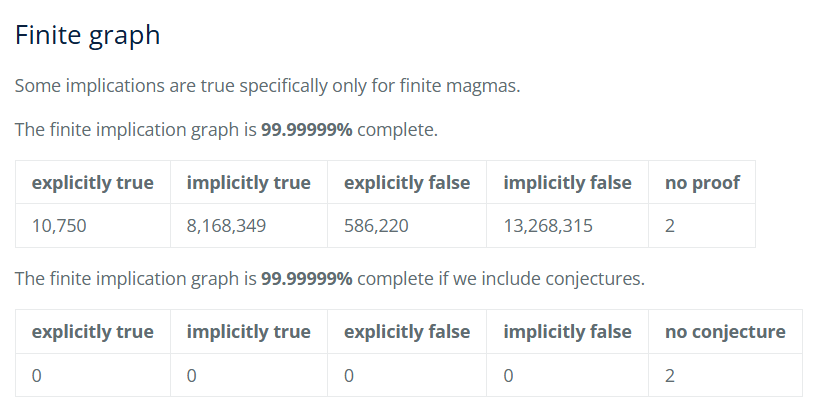
\includegraphics[width=\textwidth]{finite_status}
\end{frame}


\begin{frame}{About the project}{The Atlantic}
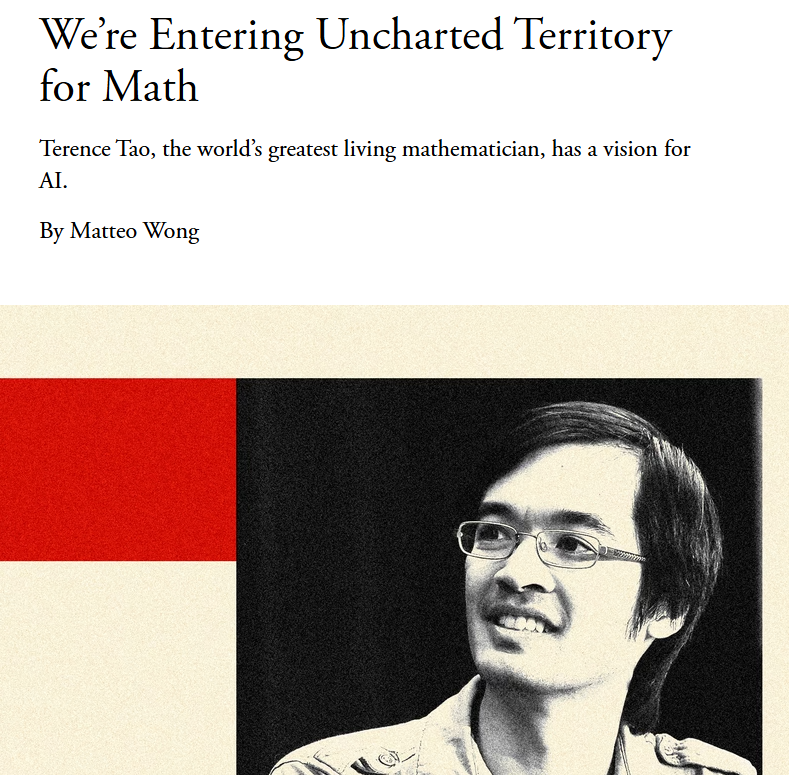
\includegraphics[width=0.7\textwidth]{atlantic}
\end{frame}


\begin{frame}{About the project}{Substack}
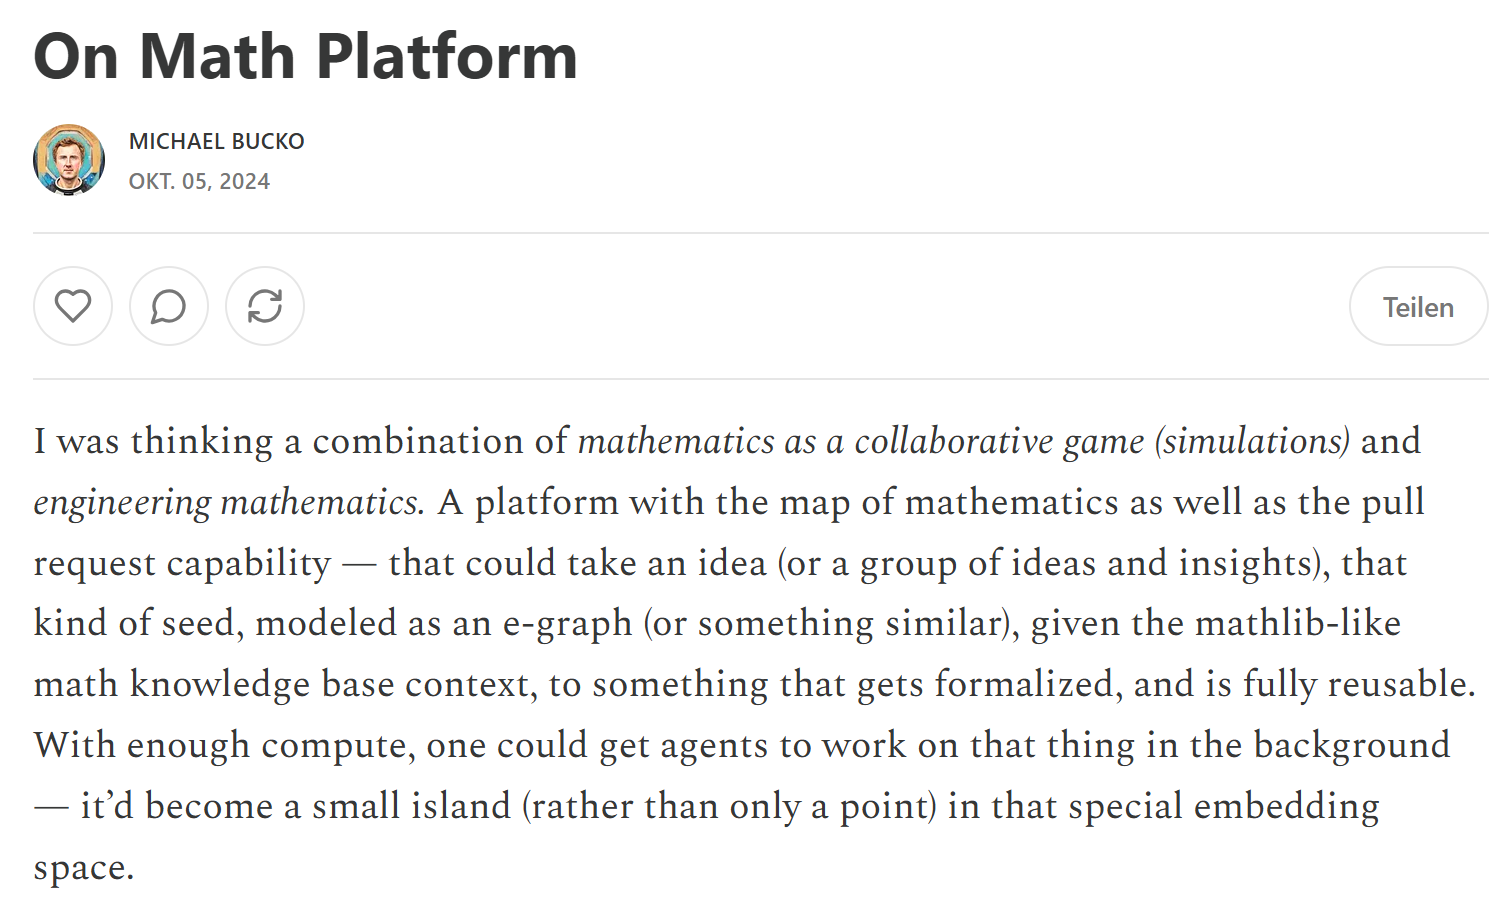
\includegraphics[width=\textwidth]{substack}
\end{frame}


\end{document}
